%%%%%%%%%%%%%%%%%%%%%%%%%%%%%%%%%%%%%%%%%%%%%%%%%%%%%%%%%%%%%%%%%%%%%%%%%%%%%%%%
% AMS Beamer series / Bologna FC / Template
% Andrea Omicini
% Alma Mater Studiorum - Università di Bologna
% mailto:andrea.omicini@unibo.it
%%%%%%%%%%%%%%%%%%%%%%%%%%%%%%%%%%%%%%%%%%%%%%%%%%%%%%%%%%%%%%%%%%%%%%%%%%%%%%%%
%\documentclass[handout]{beamer}\mode<handout>{\usetheme{default}}
%
\documentclass[presentation]{beamer}\mode<presentation>{\usetheme{AMSBolognaFC}}
%\documentclass[handout]{beamer}\mode<handout>{\usetheme{AMSBolognaFC}}
%%%%%%%%%%%%%%%%%%%%%%%%%%%%%%%%%%%%%%%%%%%%%%%%%%%%%%%%%%%%%%%%%%%%%%%%%%%%%%%%
\usepackage{ske-ski-talk-2022}
%%%%%%%%%%%%%%%%%%%%%%%%%%%%%%%%%%%%%%%%%%%%%%%%%%%%%%%%%%%%%%%%%%%%%%%%%%%%%%%%
\title[Dive into \skeski]
{Dive into \longskeski}
%
\subtitle[AMS Series Templates]
{AMS Series Templates}
%
\author[\sspeaker{Magnini}]
{\speaker{Matteo Magnini}\\\href{mailto:matteo.magnini@unibo.it}{matteo.magnini@unibo.it}}
%
\institute[DISI, Univ.\ Bologna]
{Dipartimento di Informatica -- Scienza e Ingegneria (DISI)\\\textsc{Alma Mater Studiorum} -- Universit{\`a} di Bologna}
%
\date[\today]{\today}
%
%
%%%%%%%%%%%%%%%%%%%%%%%%%%%%%%%%%%%%%%%%%%%%%%%%%%%%%%%%%%%%%%%%%%%%%%%%%%%%%%%%
\begin{document}
%%%%%%%%%%%%%%%%%%%%%%%%%%%%%%%%%%%%%%%%%%%%%%%%%%%%%%%%%%%%%%%%%%%%%%%%%%%%%%%%

%/////////
\frame{\titlepage}
%/////////

%%===============================================================================
%\section*{Outline}
%%===============================================================================
%
%%/////////
%\frame[c]{\tableofcontents[hideallsubsections]}
%%/////////


%===============================================================================
\section{Premises}
%===============================================================================

\begin{frame}[allowframebreaks]{Concerning human (and machine) reasoning}
    
    \begin{block}{The three ways}
        \begin{itemize}
            \item \alert{induction} $\rightarrow$ a kind of reasoning that uses particular examples in order to reach a general conclusion about something;
            %
            \item \alert{deduction} $\rightarrow$ the act or process of using logic or reason to form a conclusion or opinion about something;
            %
            \item \alert{abduction} $\rightarrow$ the forming and accepting on probation of a hypothesis to explain surprising facts.
        \end{itemize}
    \end{block}

    \framebreak
    
     \begin{block}{The three ways}
        \begin{itemize}
            \item \alert{induction} $\rightarrow$ machine learning (e.g., neural networks);
            %
            \item \alert{deduction} $\rightarrow$ symbolic artificial intelligence (e.g., logic programs);
            %
            \item \alert{abduction} $\rightarrow$ abductive logic programming.
        \end{itemize}
    \end{block}

    \framebreak

    %
    \begin{block}{Symbolic knowledge}
        A symbolic representation of knowledge consists of: \ccite{sub-symbolic-vs-symbolic}
        %
        \begin{enumerate}
            \item a set of symbols;
            \item\label{item:symbolic-combination} a set of grammatical rules governing the combining of symbols; 
            \item\label{item:symbolic-assignment} elementary symbols and any admissible combination of them can be assigned with meaning.
            %
            \begin{itemize}
                \item[$\Rightarrow$] Symbolic knowledge is both human and machine interpretable,
                \item first order logic (FOL) is an example of symbolic representation.
            \end{itemize}
        \end{enumerate}
    \end{block}
    
    
    \framebreak

    %/////////
    \begin{block}{Sub-symbolic data}
    \begin{itemize}
        \item ML methods, and sub-symbolic approaches in general, represent data as arrays of real numbers, and knowledge as functions over such data;
        %
        \item despite numbers are technically symbols as well, we cannot consider arrays and their functions as symbolic knowledge representation (KR) means;
        %
        \item sub-symbolic approaches frequently violate \Cref{item:symbolic-combination,item:symbolic-assignment}.
        %
    \end{itemize}
    %
    \end{block}
    %/////////
    
    \framebreak
    
    %
    \begin{block}{Local representation}
        \begin{itemize}
            \item Each number of the array has a well-defined meaning;
            %
            \item example $\rightarrow$ iris dataset sample, array with 5 elements where each element has meaning (sepal/petal length/width and class).
        \end{itemize}    
    \end{block}

    \begin{block}{Distributed representation}
        \begin{itemize}
            \item Each number of the array is meaningless, unless it is considered along with its neighbourhood;
            %
            \item example $\rightarrow$ images represented as $w\ x\ h$ matrices of numbers in range $[0,1]$.
            %
            (Violation of \cref{item:symbolic-assignment})
        \end{itemize}
    \end{block}
    
    
\end{frame}
%/////////



%===============================================================================
\section{\longski}
%===============================================================================

%/////////
\begin{frame}[allowframebreaks]{Definition}
    %
    We define \longski{} as:
    %
    \begin{displayquote}\itshape
        any \emph{algorithmic} procedure affecting how \alert{sub-symbolic predictors} draw their inferences in such a way that predictions are either \emph{computed} as a function of, or made \emph{consistent} with, some \emph{given} \alert{symbolic knowledge}*.
    \end{displayquote}
    %
    \vfill
    %
    * a wide definition that includes the vast majority of the works surveyed in \cite{surveyNeuroSymb,surveyXie,surveyCalegariCO20}.
    
\end{frame}
%/////////


%/////////
\begin{frame}[c]{Why SKI?}
    %
    There are several benefits:
    %
    \begin{itemize}
        %
        \item prevent the predictor to become a black-box\alert{!};
        %
        \item reduce learning time;
        %
        \item reduce the data size needed for training;
        %
        \item improve predictor's accuracy;
        %
        \item build a predictor that behave as a logic engine.
    \end{itemize}
    %
\end{frame}
%/////////

%/////////
\begin{frame}[c]{Explainable Artificial Intelligence \ccite{darpa2016-xai}}
    %
    Explainability can be achieved:
    %
    \begin{block}{Post-hoc explanation}
        \begin{itemize}
            \item applying an algorithm of symbolic knowledge extraction on a trained predictor;
            %
            \item output $\rightarrow$ logic rules that describe the predictor's behaviour.
            %
        \end{itemize}    
    \end{block}
    
    \begin{block}{By design}
        \begin{itemize}
            \item constraining the behaviour of predictors that are natively black-boxes with symbolic knowledge;
            %
            \item structuring the predictor's architecture with symbolic knowledge;
            %
            \item output $\rightarrow$ a predictor that does not violate the prior knowledge.
        \end{itemize}
    \end{block}
    
\end{frame}
%/////////




%===============================================================================
\section{Taxonomy}
%===============================================================================

%/////////
\begin{frame}[c]{Aim}
    %
    \begin{block}{Enrich (learning support)}
        \begin{itemize}
            \item reduce learning time;
            %
            \item reduce the data size needed for training;
            %
            \item improve predictor's accuracy.
        \end{itemize}
    \end{block}
    %
    \begin{block}{Manifold (symbolic knowledge manipulation)}
        \begin{itemize}
            \item logic inference;
            %
            \item information retrieval;
            %
            \item knowledge base completion/fusion.
        \end{itemize}
    \end{block}
\end{frame}
%/////////

%/////////
\begin{frame}[allowframebreaks]{Predictors}
    %
    Theoretically, one can inject prior knowledge into any sub-symbolic predictor.
    %
    In practice, NN are almost the sole predictors treated in literature, however, lot of different NN architecture are considered.
    %
    \begin{figure}
        \centering
        \includegraphics[width=.6\linewidth]{figures/neuron.png}
    \end{figure}
    %
    
    \framebreak
    
    \begin{figure}
        \centering
        \includegraphics[width=0.8\textwidth]{figures/cnn-architecture}
    \end{figure}
    %
    \begin{figure}
        \centering
        \includegraphics[width=0.8\textwidth]{figures/rnn-architecture}
    \end{figure}
    %
\end{frame}
%/////////


%/////////
\begin{frame}[c]{How}
    %
    There exist three major ways to perform knowledge injection on sub-symbolic predictors:
    %
    \begin{itemize}
        \item \alert{constraining}, a cost factor proportional to the violation of the knowledge is introduced during learning;
        \item \alert{structuring}, the architecture of the predictor is built in such a way to mimic the knowledge;
        \item \alert{embedding}, the symbolic knowledge is embedded into a tensor form and it is given in input as training data to the predictor.
    \end{itemize} 
    %
\end{frame}
%/////////

%/////////
\begin{frame}[allowframebreaks]{Constraining}
    %
    \begin{itemize}
        \item Knowledge cost factor is introduced in the loss function;
        %
        \item for NN the cost affects backpropagation \ccite{backpropagation} during training.
        %
        \begin{itemize}
            \item[$\Rightarrow$] Predictor does not violate the prior knowledge (to a certain extent).
        \end{itemize} 
    \end{itemize}
    
    \begin{figure}
        \centering
        \includegraphics[width=0.6\textwidth]{figures/ski-constraining}
    \end{figure}
    %
    
    \framebreak
    
    \begin{figure}
        \centering
        \includegraphics[width=0.8\textwidth]{figures/nn-backprop.png}
    \end{figure}
    
    \framebreak
    
    \begin{figure}
        \centering
        \includegraphics[width=0.8\textwidth]{figures/nn-gradient-descent.png}
    \end{figure}    
\end{frame}
%/////////

%/////////
\begin{frame}[allowframebreaks]{Structuring}
    %
    \begin{itemize}
        \item Inner architecture is shaped to be able to ``mimic'' the knowledge;
        %
        \item for NN this means \emph{ad-hoc} layers.
        %
        \begin{itemize}
            \item[$\Rightarrow$] Predictor directly exploits knowledge when needed.
        \end{itemize} 
    \end{itemize}
    %
    \begin{figure}
        \centering
        \includegraphics[width=0.7\textwidth]{figures/ski-structuring}
    \end{figure}
    %
    
    \framebreak
    
    \begin{itemize}
        \item We need to define a mapping from crispy logic rules into fuzzy continuous interpretations;
        %
        \item then we need to map the interpretations into ad-hoc neurons/layers.
    \end{itemize}   
    
    \framebreak
    
    \begin{equation*}
        \begin{aligned}
            \var{A}&\leftarrow\var{B}\wedge\var{C}\wedge\neg\var{D}.\\
            \var{A}&\leftarrow\var{E}\wedge\var{F}.\\
            \var{B}&\leftarrow\const{true}.\\
        \end{aligned}    
    \end{equation*}
    %
    \begin{figure}
        \centering
        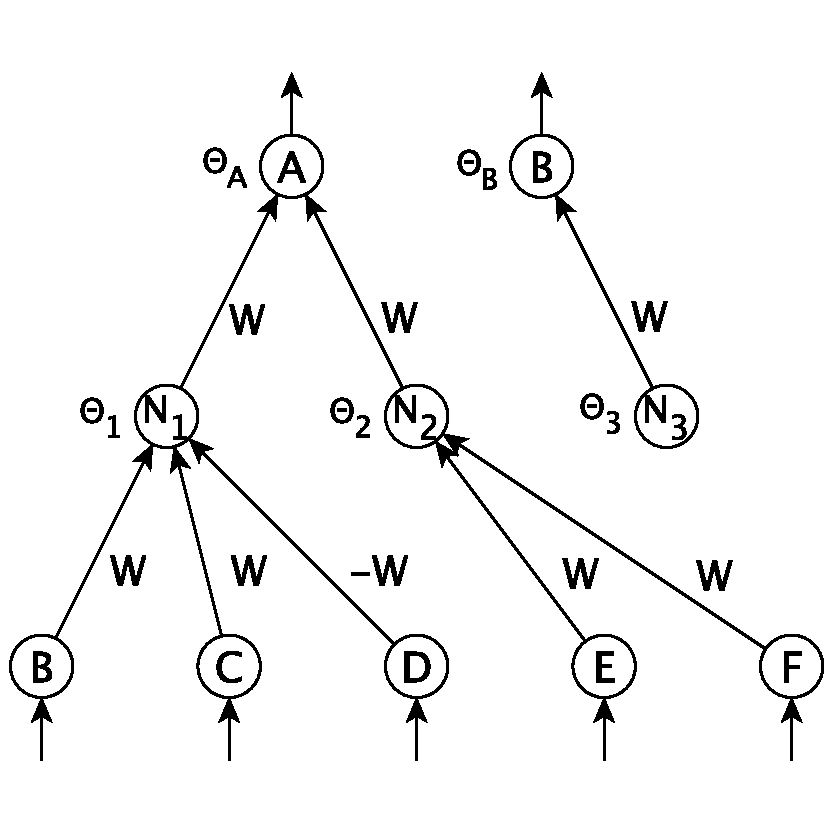
\includegraphics[height=0.5\textheight]{figures/structuring-example}
    \end{figure}
\end{frame}
%/////////

%/////////
\begin{frame}[allowframebreaks]{Embedding}
    %
    \begin{itemize}
        \item Symbolic knowledge is embedded into a tensor form;
        %
        \item this is used as predictor's input data (alone or with a ``standard'' dataset).
        %
        \begin{itemize}
            \item[$\Rightarrow$] Predictor's aim is manifold in most cases.
        \end{itemize} 
    \end{itemize}
    
    \begin{figure}
        \centering
        \includegraphics[width=0.7\textwidth]{figures/ski-embedding}
    \end{figure}
    %
    \framebreak
    %
    \begin{itemize}
        \item Knowledge graph embedding \ccite{kge-survey};
        %
        \item entities and relations are embedded into continuos vector spaces;
        %
        \item scoring function $f_{r}(h,t)$ defined on each fact $(h, r, t)$ to measure its plausibility;
    \end{itemize}
    %
    \begin{figure}
        \centering
        \includegraphics[width=0.8\textwidth]{figures/kge-space.png}
    \end{figure}
    
    \framebreak
    
    \begin{figure}
        \centering
        \includegraphics[width=0.8\textwidth]{figures/kge-nn-1.png}
    \end{figure}
    
    \begin{figure}
        \centering
        \includegraphics[width=0.8\textwidth]{figures/kge-nn-2.png}
    \end{figure}
    
\end{frame}
%/////////

%/////////
\begin{frame}[allowframebreaks]{Logic}
    \begin{block}{Intensional}
        \begin{itemize}
            \item indirect representation of data,
            %
            \item define a relation/set by describing its elements via other relations/sets.
        \end{itemize}
        %
    \end{block}
    %
    \begin{block}{Extensional}
        \begin{itemize}
            \item direct representation of data,
            %
            \item explicit definition of entities involved.
        \end{itemize}
    \end{block}
    
    Recursive intensional predicates are very expressive and powerful, as they enable the description of infinite sets via a finite (and commonly small) amount of formul\ae.
    
    \framebreak        
    
    Almost the totality of SKI algorithms deal with:
    %
    \begin{itemize}
        \item \alert{first order logic} (FOL);
        %
        \item \alert{knowledge graph} (KG);
        %
        \item \alert{propositional logic} (PL).
        
    \end{itemize}
\end{frame}
%/////////

%/////////
\begin{frame}[allowframebreaks]{First Order Logic}
    \begin{itemize}
        \item FOL is extremely flexible and expressive;
        \item you can use recursion and define recursive structures;
        \item maybe too ``powerful'' for canonic NN.
        \begin{itemize}
            \item[$\Rightarrow$] Most NN are natively DAG (directed acyclic graph)
            \item this allows backpropagation as training algorithm but ...
            \item how can you support recursion?  
        \end{itemize}
    \end{itemize}
    \centering
    %
    \phantom{You can't!}
    %
    \phantom{Unless you use some tricks.}
    
    \framebreak
    
    \begin{itemize}
        \item FOL is extremely flexible and expressive;
        \item you can use recursion and define recursive structures;
        \item maybe too ``powerful'' for canonic NN.
        \begin{itemize}
            \item[$\Rightarrow$] Most NN are natively DAG (directed acyclic graph)
            \item this allows backpropagation as training algorithm but ...
            \item how can you support recursion?  
        \end{itemize}
    \end{itemize}
    \centering
    %
    You can't!
    %
    Unless you use some tricks.
    
    \framebreak
    
    \begin{equation*}
        \begin{aligned}
            \pred{parent}(\const{abraham},\const{isaac}). &\phantom{\rightarrow} \pred{male}(\const{abraham}).\\
            \pred{parent}(\const{sarah},\const{isaac}). &\phantom{\rightarrow} \pred{female}(\const{sarah}).\\
            \pred{parent}(\const{isaac},\const{jacob}). &\phantom{\rightarrow} \pred{male}(\const{isaac}).\\
            \pred{parent}(\const{rebekah},\const{jacob}). &\phantom{\rightarrow} \pred{female}(\const{rebekah}).\\
            \dots &\phantom{\rightarrow} \pred{male}(\const{jacob}).\\
            \forall\var{X} \forall\var{Y} \pred{parent}(\const{\var{X}},\var{Y}) &\rightarrow \pred{child}(\var{Y},\var{X}).\\
            \forall\var{X} \forall\var{Y} \pred{parent}(\const{\var{X}},\var{Y}) \wedge \pred{male}(\var{X}) &\rightarrow \pred{father}(\var{X},\var{Y}).\\
            \forall\var{X} \forall\var{Y} \pred{parent}(\const{\var{X}},\var{Y}) \wedge \pred{female}(\var{X}) &\rightarrow \pred{mother}(\var{X},\var{Y}).\\
            \forall\var{X} \forall\var{Y} \exists\var{Z} \pred{parent}(\const{\var{X}},\var{Z}) \wedge \pred{parent}(\var{Z},\var{Y}) &\rightarrow \pred{grandparent}(\var{X},\var{Y}).\\
        \end{aligned}    
    \end{equation*}
\end{frame}
%/////////

%/////////
\begin{frame}[allowframebreaks]{Knowledge Graph}
    
    \begin{itemize}
        \item Only constants, variables and n-ary predicates with $n < 3$;
        \item collections of triplets $\langle \functor{a}\ \predication{f}\ \functor{b} \rangle$ or $\predication{f}(\functor{a}, \functor{b})$
        \item essentially directed graph:
        \begin{itemize}
            \item nodes $\rightarrow$ individuals,
            \item vertices $\rightarrow$ properties connecting individuals;
        \end{itemize}
        \item may instantiate an ontology, i.e., a formal description of classes characterising a given domain.
    \end{itemize}
    
    \framebreak
    
    \begin{figure}
        \centering
        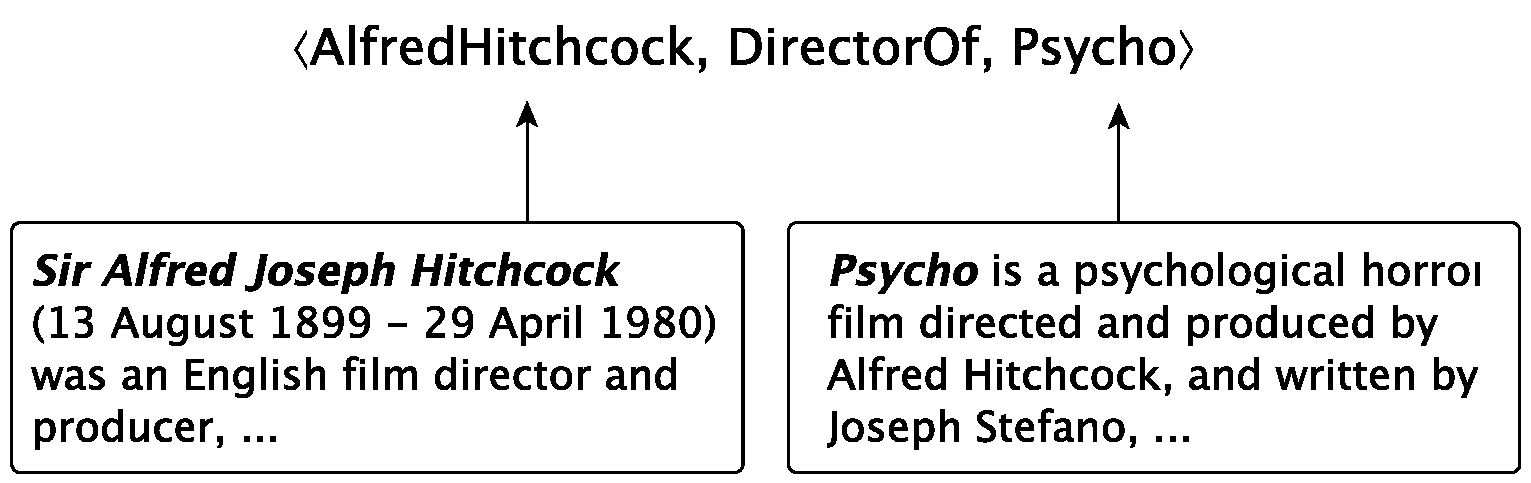
\includegraphics[width=0.8\textwidth]{figures/kg-example}
    \end{figure}    
\end{frame}    
%/////////

%/////////
\begin{frame}[allowframebreaks]{Propositional Logic}
    \begin{itemize}
        \item No quantifiers, terms, and non-atomic predicates;
        \item expressions involving one or many 0-ary predicates (propositions) possibly interconnected by ordinary logic connectives;
        \item low expressiveness, but easy to work with.
    \end{itemize}
    %
    \centering
    \begin{equation*}
        \begin{aligned}
            \pred{big\_petal}\wedge\pred{average\_sepal}&\rightarrow\const{virginica}.\\
            \pred{big\_petal}\wedge\neg\pred{average\_sepal}&\rightarrow\const{versicolor}.\\
            \pred{big\_petal}&\rightarrow\const{setosa}.\\
            \pred{average\_sepal}&\equiv(3\le\var{SepalWidth}<5)\\
            \pred{big\_petal}&\equiv(\var{PetalLength}>3)\\
        \end{aligned}    
    \end{equation*}
    
    \framebreak
    
    \begin{figure}
        \centering
        \includegraphics[width=0.6\textwidth]{figures/iris-dataset}
    \end{figure}
    
\end{frame}
%/////////


%===============================================================================
\section{Literature overview}
%===============================================================================

%/////////
\begin{frame}[c]{Notable works}
    %
    \begin{block}{KBANN: Knowledge Base Artificial Neural Network \ccite{KBANN-origin}}
        %
        It is one of the first works in SKI.
        %
        Authors inject prior knowledge into a NN and validate their method on real world biological datasets.
        %
        \begin{itemize}
            %
            \item aim $\rightarrow$ enrich;
            %
            \item predictor $\rightarrow$ neural network;
            %
            \item how $\rightarrow$ structuring and constraining;
            %
            \item logic $\rightarrow$ propositional.
            %    
        \end{itemize}        
    \end{block}
    %
\end{frame}
%/////////

%/////////
\begin{frame}[allowframebreaks]{KBANN}
    \begin{block}{Algprithm}
        \begin{enumerate}
            \item rewrite rules so that disjuncts are expressed as a set of rules that each have only one antecedent;
            %
            \item directly map the rule structure into a neural network;
            %
            \item label units in the KBANN-net according to their ``level'';
            %
            \item add hidden units to the network at user-specified levels (optional);
            %
            \item add units for known input features that are not referenced in the rules;
            %
            \item add links not specified by translation between all units in topologically-contiguous levels;
            %
            \item Perturb the network by adding near-zero random numbers to all link weights and biases.
        \end{enumerate}
    \end{block}
    
    \framebreak
    
    \begin{figure}
        \centering
        \includegraphics[width=0.7\textwidth]{figures/kbann-algorithm.png}
    \end{figure}
    
    \framebreak
    
    \begin{equation*}
        \begin{aligned}
            \textit{Error}&= - \sum_{i=1}^{n}{[(1-d_{i})*\log_{2}{(1-a_{i})} + d_{i}*\log_{2}{(a_{i})}]}\\
            \textit{Regularizer}&=\lambda\sum_{i\in\omega}{\frac{(\omega_{i} - \omega_{init_{i}})^{2}}{1+(\omega_{i}- \omega_{init_{i}})^{2}}}
        \end{aligned}
    \end{equation*}
\end{frame}
%/////////

%/////////
\begin{frame}[allowframebreaks]{FANN}
    %
    \begin{block}{FANN: Fibred Artificial Neural Network \ccite{FANN-theory,BaderFlairs2005}}
        %
        Authors present an interesting approach to deal with FOL in NN.
        %
        The key idea is to allow single neurons to behave like entire embedded networks according to a fibring function $\phi$.
        %
        \begin{itemize}
            %
            \item aim $\rightarrow$ manifold;
            %
            \item predictor $\rightarrow$ neural network;
            %
            \item how $\rightarrow$ structuring;
            %
            \item logic $\rightarrow$ first order logic.
            %    
        \end{itemize}        
    \end{block}
    
    \framebreak
    
    \begin{figure}
        \centering
        \includegraphics[height=0.8\textheight]{figures/fibring-example.png}
    \end{figure}
    
\end{frame}
%/////////

%===============================================================================
\section{\longpsyki}
%===============================================================================

%/////////
\begin{frame}{General SKI workflow}
    
    \begin{figure}
        \centering
        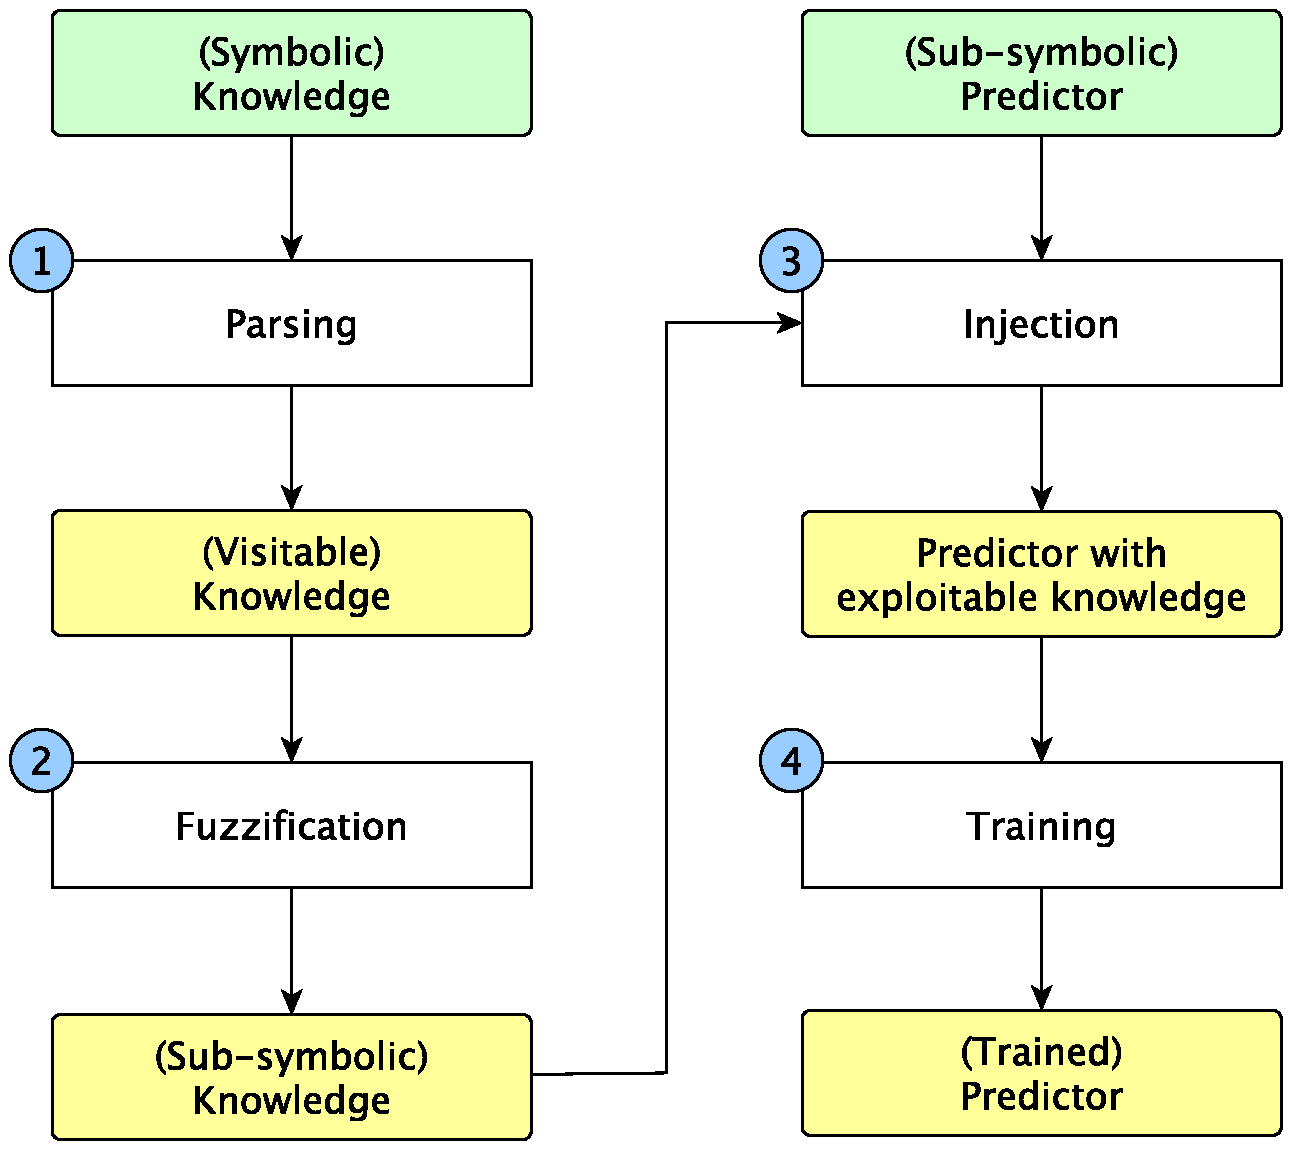
\includegraphics[width=0.8\textheight]{figures/ski-workflow.pdf}
    \end{figure}
    
\end{frame}
%/////////

%\\\\\\\\
\begin{frame}{1 -- Parsing}
    
    \begin{minipage}{0.5\textwidth}
        \begin{equation*}
            \begin{split}
                class&(X_{-30}, \dots, X_{30}, ie) \leftarrow\\
                &\textit{pyramidine-rich}(\dots)\ \wedge\\
                &X_{-3} = y\ \wedge\\
                &X_{-2} = a\ \wedge\\
                &X_{-1} = g\ \wedge\\
                &X_{1} = g\ \wedge\\
                &\neg(\textit{ie-stop}(\dots)) 
            \end{split}
        \end{equation*}
    \end{minipage}
    \noindent\begin{minipage}{0.4\textwidth}% adapt widths of minipages to your needs
        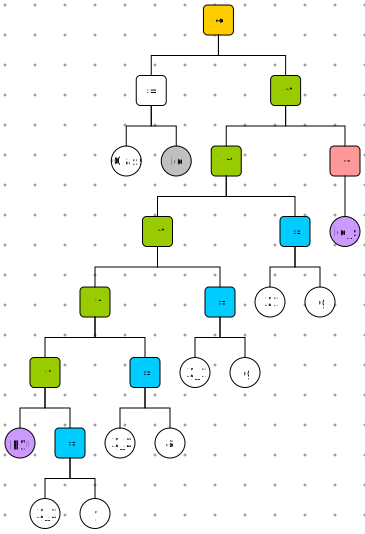
\includegraphics[width=\linewidth]{figures/ast-ie-1.png}
    \end{minipage}%
    
    
\end{frame}
%\\\\\\\\\\\\\\\\\\\\\

%\\\\\\\\\\\\\\\\\\\\\
\begin{frame}{2 -- Fuzzification}
    
    \begin{minipage}{0.6\textwidth}
        % !TeX spellcheck = en_GB
% !TeX root = ../ski-extraamas-2022.tex

\centering
\begin{adjustbox}{width=\textwidth,totalheight=0.7\textheight,keepaspectratio}
%\begin{table}%[!h]
    %
    \begin{tabular}{l|r}
        \textbf{Formula} & \textbf{Continuous interpretation}
        \\
        \hline\hline
        $\llbracket\neg \phi\rrbracket$ & $1 - \llbracket\phi\rrbracket$
        \\
        $\llbracket\phi  \wedge \psi\rrbracket$ &  $min\{\llbracket\phi\rrbracket, \llbracket\psi\rrbracket\}$
        \\
        $\llbracket\phi  \vee \psi\rrbracket$ & $max\{\llbracket\phi\rrbracket, \llbracket\psi\rrbracket\}$
        \\
        $\llbracket\phi = \psi\rrbracket$ & $\llbracket\neg( \phi \ne \psi )\rrbracket $
        \\
        $\llbracket\phi \ne \psi\rrbracket$ & $|\llbracket\phi\rrbracket-\llbracket\psi\rrbracket|$ 
        \\
        $\llbracket\phi > \psi\rrbracket$  & $max\{0, \llbracket\phi\rrbracket - \llbracket\psi\rrbracket\}$
        \\
        $\llbracket\phi \ge \psi\rrbracket$ & $\llbracket( \phi > \psi ) \vee ( \phi = \psi )\rrbracket$ 
        \\
        $\llbracket\phi < \psi\rrbracket$  &  $max\{0, \llbracket\psi\rrbracket - \llbracket\phi\rrbracket\}$
        \\
        $\llbracket\phi \le \psi\rrbracket$  & $\llbracket( \phi < \psi ) \vee ( \phi = \psi )\rrbracket$
        \\
        $\llbracket\phi \Rightarrow \psi\rrbracket$ & $min\{1, 1- \llbracket\psi\rrbracket+\llbracket\phi\rrbracket\}$
         \\
        $\llbracket\phi \Leftarrow \psi\rrbracket$ & $min\{1, 1-\llbracket\phi\rrbracket+\llbracket\psi\rrbracket\}$ 
        \\
        $\llbracket\phi \Leftrightarrow \psi\rrbracket$ & $min\{1, 1-|\llbracket\phi\rrbracket-\llbracket\psi\rrbracket|\}$ 
        \\
        $\llbracket \text{expr}(\bar{X}) \rrbracket$ & $\text{expr}(\llbracket\bar{X}\rrbracket)$
        \\
        $\llbracket \mathtt{true} \rrbracket$ & $1$
        \\
        $\llbracket \mathtt{false} \rrbracket$ & $0$
        \\
        $\llbracket X \rrbracket$ & $x$
        \\
        $\llbracket \const{k} \rrbracket$ & $k$
        \\
        $\llbracket \pred{p}(\bar{X}) \rrbracket^{**}$ & $\llbracket \psi_1 \vee \ldots \vee \psi_k \rrbracket$
        \\
        $\llbracket \pred{class}(\bar{X}, \const{y}_i) \leftarrow \psi \rrbracket$ & $\llbracket \psi \rrbracket^{*}$
    \end{tabular}
%\end{table}
\end{adjustbox}
        
        \begin{center}\scriptsize
            $^{*}$ encodes the value for the $i^{th}$ output
            \\
            \smallskip
            $^{**}$ assuming $p$ is defined by $k$ clauses of the form:
            \\
            $\pred{p}(\bar{X}) \leftarrow \psi_1,\ \ldots,\ \pred{p}(\bar{X}) \leftarrow \psi_k$
        \end{center}
    \end{minipage}
    %
    \begin{minipage}{0.35\textwidth}
        \begin{equation*}
            \begin{split}
                class&(X_{-30}, \dots, X_{30}, ie) \leftarrow\\
                &X_{-3} = y\ \wedge\\
                &X_{-2} = a\ \wedge\\
                &X_{-1} = g\ \wedge\\
                &X_{1} = g
            \end{split}
        \end{equation*}
        %
        \centering
        $\downarrow$
        \begin{equation*}
            \begin{split}
                min\{&min\{min\{1-|X_{-3} - y|,\\
                &\phantom{min\{min\{}1-|X_{-2} - a|\},\\
                &\phantom{min\{}1-|X_{-1} - g|\},\\
                &1-|X_{1}-g|\}
            \end{split}
        \end{equation*}
    \end{minipage}
    
\end{frame}
%\\\\\\\\\\\\\\\\\\\\\

%/////////
\begin{frame}[c]{3 -- Injection}
    %
    Injection step is algorithm specific but it falls back into the three approaches already discussed:
    \begin{block}{Injection families}
        \begin{itemize}
            \item constraining;
            \item structuring;
            \item embedding.
        \end{itemize}
    \end{block}
    %
    We will see some examples later.
\end{frame}
%/////////

%/////////
\begin{frame}[c]{4 -- Training}
    %
    \begin{figure}
        \centering
        \includegraphics[width=0.8\textwidth]{figures/training-workflow.png}
    \end{figure}
\end{frame}
%/////////


%/////////
\begin{frame}[allowframebreaks]{Overall Design}
    \begin{figure}
        \centering
        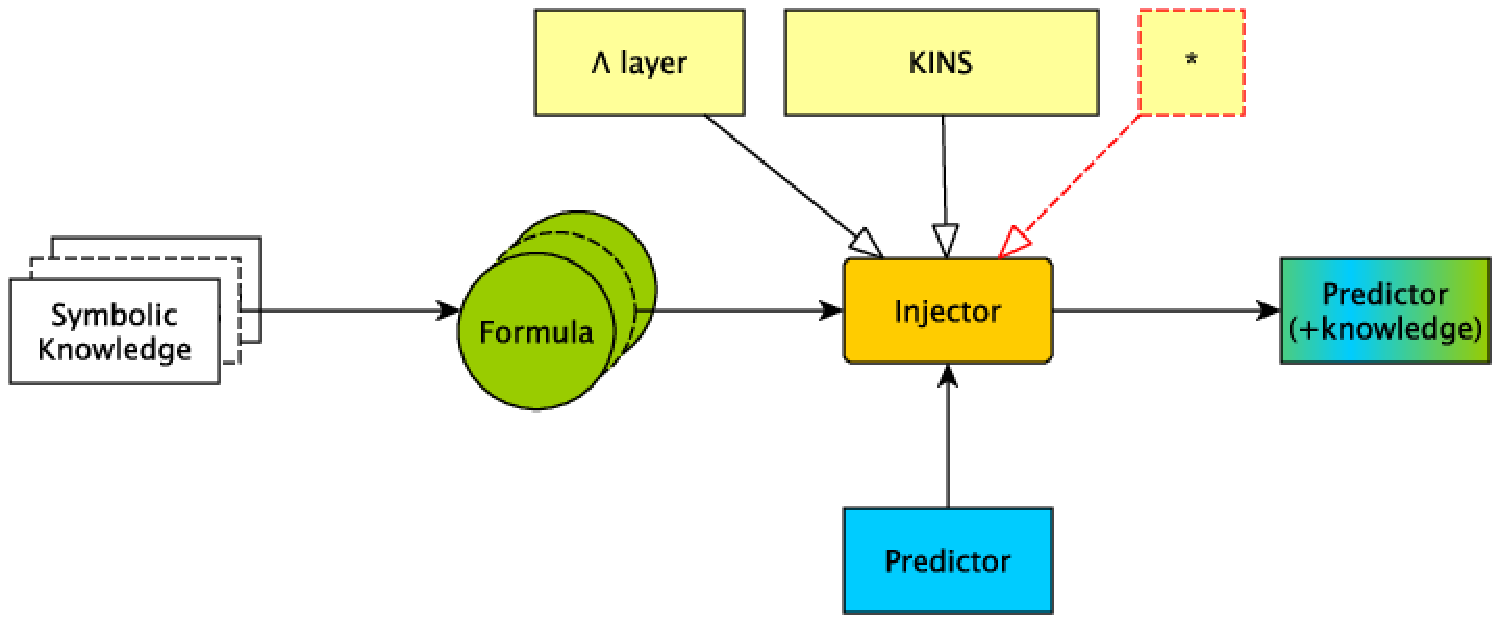
\includegraphics[width=0.8\textwidth]{figures/psyki-design}
    \end{figure}
    
    \framebreak
    
    \begin{figure}
        \centering
        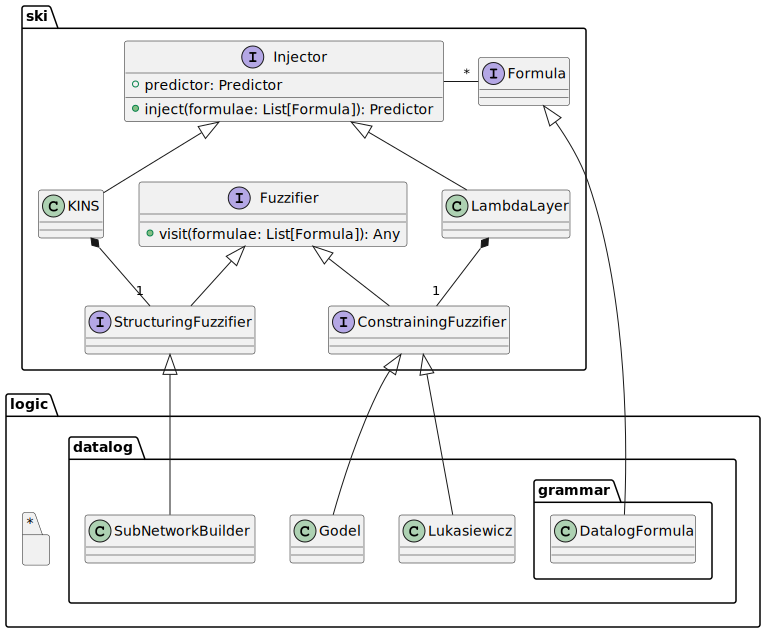
\includegraphics[height=0.8\textheight]{figures/psyki-class-diagram}
    \end{figure}
    
    \framebreak
    
    \begin{block}{Key components}
        \begin{itemize}
            \item\alert{injector}: an entity capable of injecting symbolic knowledge into sub-symbolic predictors;
            %
            \item\alert{predictor}: a classifier/regressor;
            %
            \item\alert{formula}: a visitable data structure representing a logic rule;
            %
            \item\alert{fuzzifier}: an entity that embed a crisp formula into a fuzzy continuous interpretation object.
        \end{itemize}
    \end{block}
\end{frame}
%/////////


%/////////
\begin{frame}[allowframebreaks]{Knowledge Injection via Network Structuring}
    
    \begin{block}{KINS: Knowledge Injection via Network Structuring}
        %
        A general SKI algorithm that does not impose constrains on the sub-symbolic predictor to enrich.
        %
        \begin{itemize}
            %
            \item aim $\rightarrow$ enrich;
            %
            \item predictor $\rightarrow$ neural network;
            %
            \item how $\rightarrow$ structuring;
            %
            \item logic $\rightarrow$ stratified Datalog with negation.
            %    
        \end{itemize}        
    \end{block}
    
    \framebreak
    
    \begin{figure}
        \centering
        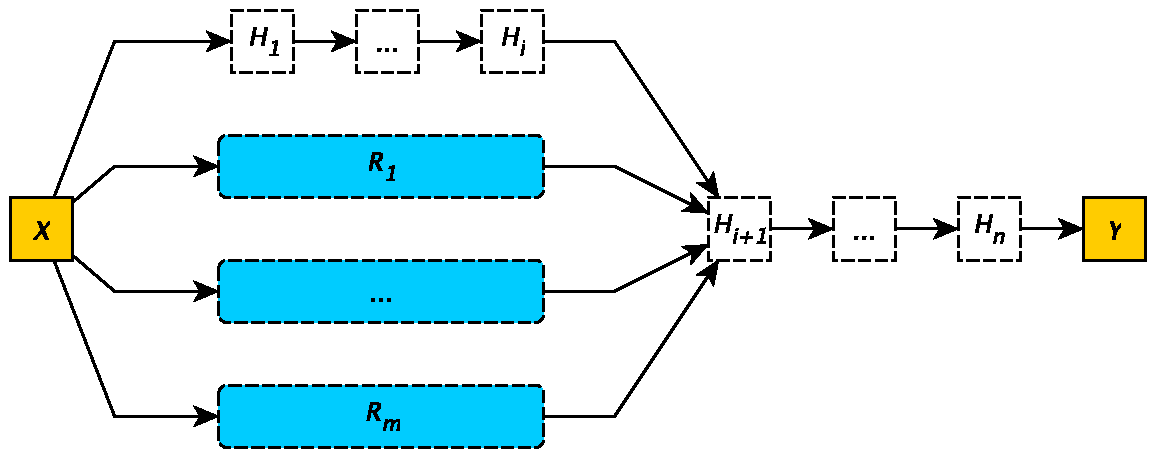
\includegraphics[width=0.8\textwidth]{figures/kins-architecture}
    \end{figure}
    
    \framebreak
    
    \resizebox{\textwidth}{!}{
    \begin{tabular}{l|r||cl|r}
         \textbf{Formula} & \textbf{C. interpretation} & & \textbf{Formula} & \textbf{C. interpretation}
        \\
        \hline\hline
        $\llbracket\neg \phi\rrbracket$ & $\eta(1 - \llbracket\phi\rrbracket)$ & & $\llbracket\phi \le \psi\rrbracket$  & $\eta(1 + \llbracket \psi \rrbracket - \llbracket \phi \rrbracket)$  % Negation % Less equal
        \\
        $\llbracket\phi  \wedge \psi\rrbracket$ &  $\eta(min(\llbracket\phi\rrbracket, \llbracket\psi\rrbracket))$ & &  $\llbracket \pred{class}(\bar{X}, \const{y}_i) \leftarrow \psi \rrbracket$ & $\llbracket \psi \rrbracket^{*}$ % Conjunction % Class
        \\
        $\llbracket\phi  \vee \psi\rrbracket$ & $\eta(max(\llbracket\phi\rrbracket, \llbracket\psi\rrbracket))$ & & $\llbracket \text{expr}(\bar{X}) \rrbracket$ & $\text{expr}(\llbracket\bar{X}\rrbracket)$ % Disjunction
        \\
        $\llbracket\phi = \psi\rrbracket$ & $\eta(\llbracket\neg( \phi \ne \psi )\rrbracket )$ & &$\llbracket \mathtt{true} \rrbracket$ & $1$ % Equal
        \\
        $\llbracket\phi \ne \psi\rrbracket$ & $\eta(|\llbracket\phi\rrbracket-\llbracket\psi\rrbracket|)$ & & $\llbracket \mathtt{false} \rrbracket$ & $0$ % Not Equal
        \\
        $\llbracket\phi > \psi\rrbracket$ & $\eta(max(0, \frac{1}{2} + \llbracket\phi\rrbracket - \llbracket\psi\rrbracket))$ & & $\llbracket X \rrbracket$ & $x$ % Greater
        \\
        $\llbracket\phi \ge \psi\rrbracket$  & $\eta(1 + \llbracket \phi \rrbracket - \llbracket \psi \rrbracket)$ & & $\llbracket \const{k} \rrbracket$ & $k$ % Greater Equal
        \\
        $\llbracket\phi < \psi\rrbracket$  &  $\eta(max(0, \frac{1}{2} + \llbracket\psi\rrbracket - \llbracket\phi\rrbracket))$ & & $\llbracket \pred{p}(\bar{X}) \rrbracket^{**}$ & $\llbracket \psi_1 \vee \ldots \vee \psi_k \rrbracket$ % Less       
    \end{tabular}
}
\begin{center}\scriptsize
    $^{*}$ encodes the value for the $i^{th}$ output
    \\
    \smallskip
    $^{**}$ assuming $p$ is defined by $k$ clauses of the form:
    \\
    $\pred{p}(\bar{X}) \leftarrow \psi_1,\ \ldots,\ \pred{p}(\bar{X}) \leftarrow \psi_k$
\end{center}
    
    \framebreak
    
    \begin{figure}
        \centering
        \includegraphics[width=0.8\textwidth]{figures/kins-fuzzifier-modules}
    \end{figure}
    
\end{frame}
%/////////

%/////////
\begin{frame}[fragile,allowframebreaks]{Case study}
    %
    PSJGS: Primate Splice-Junction Gene Sequences dataset
    %
    \begin{minipage}{0.5\textwidth}
        \begin{lstlisting}[language={}, basicstyle=\ttfamily\tiny,frame=none]
            EI-stop ::- @-3 'TAA'.
            EI-stop ::- @-3 'TAG'.
            EI-stop ::- @-3 'TGA'.
            EI-stop ::- @-4 'TAA'.
            EI-stop ::- @-4 'TAG'.
            EI-stop ::- @-4 'TGA'.
            EI-stop ::- @-5 'TAA'.
            EI-stop ::- @-5 'TAG'.
            EI-stop ::- @-5 'TGA'.
            
            IE-stop ::- @1 'TAA'.
            IE-stop ::- @1 'TAG'.
            IE-stop ::- @1 'TGA'.
            IE-stop ::- @2 'TAA'.
            IE-stop ::- @2 'TAG'.
            IE-stop ::- @2 'TGA'.
            IE-stop ::- @3 'TAA'.
            IE-stop ::- @3 'TAG'.
            IE-stop ::- @3 'TGA'.
            
            pyramidine-rich :- 6 of (@-15 'YYYYYYYYYY').
            
            EI :- @-3 'MAGGTRAGT', not(EI-stop).
            
            IE :- pyramidine-rich, @-3 'YAGG', not(IE-stop).
        \end{lstlisting}
    \end{minipage}
    \vline
    \begin{minipage}{0.45\textwidth}
        \begin{lstlisting}[language={}, basicstyle=\ttfamily\tiny,frame=none]           
            Class, Id, DNA-sequence
            
            EI,ATRINS-DONOR-521,CCAGCTGCAT...AGCCAGTCTG
            EI,ATRINS-DONOR-905,AGACCCGCCG...GTGCCCCCGC
            EI,BABAPOE-DONOR-30,GAGGTGAAGG...CACGGGGATG
            ...
            IE,ATRINS-ACCEPTOR-701,TTCAGCGGCC...GCCCTGTGGA
            IE,ATRINS-ACCEPTOR-1678,GGACCTGCTC...GGGGGCTCTA
            IE,BABAPOE-ACCEPTOR-801,GCGGTTGATT...AAGATGAAGG
            ...
            N,AGMKPNRSB-NEG-1,CAAAAGAACA...CAAGGCTACA
            N,AGMORS12A-NEG-181,AGGGAGGTGT...GGGCATGGGG
            N,AGMORS9A-NEG-481,TGGTCAATTC...TCTTGCTCTG
            ...
            
            3190 Records
        \end{lstlisting}
    \end{minipage}
    
    \framebreak
    
    \centering
\resizebox*{!}{0.8\textheight}{
    \centering
    \begin{adjustbox}{width=\linewidth, center}
        \centering
        \begin{tabular}{c|l}
            \centering
            \textbf{Class} & \textbf{Logic Formulation}
            \\\hline\hline
            \emph{EI} & $\begin{array}{l}
                \begin{aligned}
                    \pred{class}(\bar{\var{X}}, \const{ei}) \leftarrow& \var{X}_{-3} = \const{m} \wedge \var{X}_{-2} = \const{a} \wedge \var{X}_{-1} = \const{g} \wedge \var{X}_{+1} = \const{g}\ \wedge\\
                    & \var{X}_{+2} = \const{t} \wedge \var{X}_{+3} = \const{a} = \const{r} \wedge \var{X}_{+4} = \const{a}\ \wedge \\
                    & \var{X}_{+5} = \const{g} \wedge \var{X}_{+6} = \const{t} \wedge \neg(\pred{ei\_stop}(\bar{\var{X}}))
                \end{aligned}
                \\
                \pred{ei\_stop}(\bar{\var{X}}) \leftarrow \var{X}_{-3} = \const{t} \wedge \var{X}_{-2} = \const{a} \wedge \var{X}_{-1} = \const{a}
                \\
                \pred{ei\_stop}(\bar{\var{X}}) \leftarrow \var{X}_{-3} = \const{t} \wedge \var{X}_{-2} = \const{a} \wedge \var{X}_{-1} = \const{g}
                \\
                \pred{ei\_stop}(\bar{\var{X}}) \leftarrow \var{X}_{-3} = \const{t} \wedge \var{X}_{-2} = \const{g} \wedge \var{X}_{-1} = \const{a}
                \\
                \pred{ei\_stop}(\bar{\var{X}}) \leftarrow \var{X}_{-4} = \const{t} \wedge \var{X}_{-3} = \const{a} \wedge \var{X}_{-2} = \const{a}
                \\
                \pred{ei\_stop}(\bar{\var{X}}) \leftarrow \var{X}_{-4} = \const{t} \wedge \var{X}_{-3} = \const{a} \wedge \var{X}_{-2} = \const{g}
                \\
                \pred{ei\_stop}(\bar{\var{X}}) \leftarrow \var{X}_{-4} = \const{t} \wedge \var{X}_{-3} = \const{g} \wedge \var{X}_{-2} = \const{a}
                \\
                \pred{ei\_stop}(\bar{\var{X}}) \leftarrow \var{X}_{-5} = \const{t} \wedge \var{X}_{-4} = \const{a} \wedge \var{X}_{-3} = \const{a}
                \\
                \pred{ei\_stop}(\bar{\var{X}}) \leftarrow \var{X}_{-5} = \const{t} \wedge \var{X}_{-4} = \const{a} \wedge \var{X}_{-3} = \const{g}
                \\
                \pred{ei\_stop}(\bar{\var{X}}) \leftarrow \var{X}_{-5} = \const{t} \wedge \var{X}_{-4} = \const{g} \wedge \var{X}_{-3} = \const{a}
            \end{array}$
            \\\hdashline
            \emph{IE} & $\begin{array}{l}
                \begin{aligned}
                    \pred{class}(\bar{\var{X}}, \const{ie}) \leftarrow &\pred{pyramidine\_rich}(\bar{\var{X}}) \wedge \neg(\pred{ie\_stop}(\bar{\var{X}}))\ \wedge\\
                    & \var{X}_{-3} = \const{y} \wedge \var{X}_{-2} = \const{a} \wedge \var{X}_{-1} = \const{g} \wedge \var{X}_{+1} = \const{g}
                \end{aligned}
                \\
                \pred{pyramidine\_rich}(\bar{\var{X}}) \leftarrow 6 \le (\var{X}_{-15} = \const{y} + \ldots + \var{X}_{-6} = \const{y})
                \\
                \pred{ie\_stop}(\bar{\var{X}}) \leftarrow \var{X}_{+2} = \const{t} \wedge \var{X}_{+3} = \const{a} \wedge \var{X}_{+4} = \const{a}
                \\
                \pred{ie\_stop}(\bar{\var{X}}) \leftarrow \var{X}_{+2} = \const{t} \wedge \var{X}_{+3} = \const{a} \wedge \var{X}_{+4} = \const{g}
                \\
                \pred{ie\_stop}(\bar{\var{X}}) \leftarrow \var{X}_{+2} = \const{t} \wedge \var{X}_{+3} = \const{g} \wedge \var{X}_{+4} = \const{a}
                \\
                \pred{ie\_stop}(\bar{\var{X}}) \leftarrow \var{X}_{+3} = \const{t} \wedge \var{X}_{+4} = \const{a} \wedge \var{X}_{+5} = \const{a}
                \\
                \pred{ie\_stop}(\bar{\var{X}}) \leftarrow \var{X}_{+3} = \const{t} \wedge \var{X}_{+4} = \const{a} \wedge \var{X}_{+5} = \const{g}
                \\
                \pred{ie\_stop}(\bar{\var{X}}) \leftarrow \var{X}_{+3} = \const{t} \wedge \var{X}_{+4} = \const{g} \wedge \var{X}_{+5} = \const{a}
                \\
                \pred{ie\_stop}(\bar{\var{X}}) \leftarrow \var{X}_{+4} = \const{t} \wedge \var{X}_{+5} = \const{a} \wedge \var{X}_{+6} = \const{a}
                \\
                \pred{ie\_stop}(\bar{\var{X}}) \leftarrow \var{X}_{+4} = \const{t} \wedge \var{X}_{+5} = \const{a} \wedge \var{X}_{+6} = \const{g}
                \\
                \pred{ie\_stop}(\bar{\var{X}}) \leftarrow \var{X}_{+4} = \const{t} \wedge \var{X}_{+5} = \const{g} \wedge \var{X}_{+6} = \const{a}
            \end{array}$
        \end{tabular}
    \end{adjustbox}
}

    
    \framebreak
    
    \begin{figure}
        \centering
        \includegraphics[width=0.6\textwidth]{figures/dna-rules-confusion-matrix}
    \end{figure}
    %
    
    \framebreak
    
    \begin{figure}
        \centering
        \includegraphics[width=\textwidth]{figures/kins-error-rate}
    \end{figure}
    %
    
\end{frame}
%/////////


%===============================================================================
\section{Open literature research lines}
%===============================================================================


%/////////
\begin{frame}[c]{SKE \& SKI}
    %
    \begin{figure}
        \centering
        \includegraphics[width=\textwidth]{figures/ske-ski-workflow}
    \end{figure}
\end{frame}
%/////////


%/////////
\begin{frame}[c]{Multi-Agent Systems}
    %
    \begin{itemize}
        \item agent to agent explanation \ccite{explanation-aixia2020dp}\\
        %
        $\rightarrow$ SKE + SKI + explanation;
        %
        \item logic as lingua franca for communication between heterogeneous entities;
        %
        \item knowledge sharing and knowledge exploitation among agents;
        %
        \item symbolic techniques integrated with sub-symbolic ones\\
        %
        $\rightarrow$ representing and manipulating cognitive
        processes and their results.
    \end{itemize}
\end{frame}
%/////////

%===============================================================================
\section*{}
%===============================================================================

%/////////
\frame{\titlepage}
%/////////

%===============================================================================
\section*{\refname}
%===============================================================================

%%%%
\setbeamertemplate{page number in head/foot}{}
%/////////
%\begin{frame}[c,noframenumbering]{\refname}
\begin{frame}[t,allowframebreaks,noframenumbering]{\refname}
    %	\tiny
    \scriptsize
    %	\footnotesize
    \bibliographystyle{apalike-AMS}
    \bibliography{ske-ski-talk-2022}
\end{frame}
%/////////

%%%%%%%%%%%%%%%%%%%%%%%%%%%%%%%%%%%%%%%%%%%%%%%%%%%%%%%%%%%%%%%%%%%%%%%%%%%%%%%%
\end{document}
%%%%%%%%%%%%%%%%%%%%%%%%%%%%%%%%%%%%%%%%%%%%%%%%%%%%%%%%%%%%%%%%%%%%%%%%%%%%%%%%
